%% Einleitung

\begin{tabularx}{\textwidth}{Xr}
  Constantin Lazari, Marco Wettstein & \today\\
\end{tabularx}

%% Fragen
\begin{questions}
  \question
  Geben Sie je eine \textbf{\textit{kfG}} f�r die folgenden Sprachen an: 

	\begin{parts}
		\part $\{a^nb^{n+k}a^k | n, k > 0\}$
		\begin{solutionordottedlines}[2cm]
		\begin{align*}
			R & \rightarrow bRa\\
			R & \rightarrow ba\\
			L & \rightarrow aLb\\
			L & \rightarrow ab\\
			L & \rightarrow LR
		\end{align*}
		\end{solutionordottedlines}

		\part $\{a^nb^{n+2} | n > 0\}$
		\begin{solutionordottedlines}[2cm]
		\begin{align*}
			A & \rightarrow abbb\\
			A & \rightarrow aAb
		\end{align*}
		\end{solutionordottedlines}
	\end{parts}

   %%%%%%%%%%%%%%%%%%%%%%%%%%%%%%%%%%%%%%%%%%%%%%%%%%%%
	
	\question
	Gegeben sei die in der Vorlesung verwendete \textbf{\textit{kfG}}
	\begin{equation*}
		G_A = (V,T,P,S) = (\{A,B\},\{+,*,a-z,0-9,(,)\},P,A)
	\end{equation*}
	f�r (vereinfachte) Ausdr�cke in Programmiersprachen.

	\begin{parts}
		\part Zeigen Sie, $w \in L(G_A)$ mit $w = ((a+d) * (cd1 + (e * d2)))$ gilt.
		\begin{solutionordottedlines}[2cm]
		\begin{align*}
			A	& \rightarrow  (A) \rightarrow (A * A) \rightarrow ((A) * A) \rightarrow ((A + A) * A) \\
				& \rightarrow ((B + B) * A) \rightarrow ((a + d) * A) \rightarrow ((a + d) * (A))\\
				& \rightarrow ((a + d) * (A + A)) \rightarrow ((a + d) * (B + A)) \rightarrow ((a + d) * (B1 + A)) \\
				& \rightarrow ((a + d) * (Bd1 + A)) \rightarrow ((a + d) * (cd1 + A)) \\
				& \rightarrow ((a + d) * (cd1 + (A)))  \rightarrow ((a + d) * (cd1 + (A * A))) \\
				& \rightarrow ((a + d) * (cd1 + (B * A))) \rightarrow ((a + d) * (cd1 + (e * A)))\\ 
				& \rightarrow ((a + d) * (cd1 + (e * B))) \rightarrow ((a + d) * (cd1 + (e * B2)))\\ 
				& \rightarrow ((a + d) * (cd1 + (e * d2))) = w
		\end{align*}
		$w$ l�sst sich also erzeugen, somit ist $w$ ein g�ltiges Wort.
		\end{solutionordottedlines}

		\pagebreak
		\part Geben Sie f�r $w = (a11 * e) + (c + (a * d2))$ die links- und rechtsseitigen Ableitungen an
		\begin{solutionordottedlines}[2cm]
			Um die Sache zu verk�rzen haben wir $A \rightarrow B$ f�r alle $A$ auf einmal durchgef�hrt.
		\begin{enumerate}
			\item linksseitig
			\begin{align*}
				A & \rightarrow A + A \rightarrow (A) + A \rightarrow (A * A) + A \rightarrow (A * A) + (A)\\
				& \rightarrow (A * A) + (A + A) \rightarrow (A * A) + (A + (A))\\
				& \rightarrow (A * A) + (A + (A * A)) \rightarrow (B * A) + (A + (A * A))\\
				& \rightarrow (B * B) + (B + (B * B)) \rightarrow (aB * B) + (B + (B * B))\\
				& \rightarrow (a1B * B) + (B + (B * B)) \rightarrow (a11 * B) + (B + (B * B))\\
				& \rightarrow (a11 * e) + (B + (B * B)) \rightarrow (a11 * e) + (c + (B * B))\\
				& \rightarrow (a11 * e) + (c + (a * B)) \rightarrow (a11 * e) + (c + (a * dB))\\
				& \rightarrow (a11 * e) + (c + (a * d2))
			\end{align*}
			\item rechtsseitig
			\begin{align*}
				A & \rightarrow (A) \rightarrow (A * A) \rightarrow A + (A * A) \rightarrow (A + (A * A))\\
				& \rightarrow A + (A + (A * A)) \rightarrow (A) + (A + (A * A))\\
				& \rightarrow (A * A) + (A + (A * A)) \rightarrow (B * B) + (B + (B * B))\\ 
				& \rightarrow (B * B) + (B + (B * B2)) \rightarrow (B * B) + (B + (B * d2))\\
				& \rightarrow (B * B) + (B + (a * d2)) \rightarrow (B * B) + (c + (a * d2))\\
				& \rightarrow (B * e) + (c + (a * d2)) \rightarrow (B1 * e) + (c + (a * d2))\\
				& \rightarrow (B11 * e) + (c + (a * d2)) \rightarrow (a11 * e) + (c + (a * d2))
			\end{align*}
		\end{enumerate}
		\end{solutionordottedlines}
	\end{parts}

   %%%%%%%%%%%%%%%%%%%%%%%%%%%%%%%%%%%%%%%%%%%%%%%%%%%%
	\pagebreak
	\question
	Gegeben sei die  \textbf{\textit{kfG}} $G_{Auf} = (V,T,P,S) = (\{S\}, \{\epsilon, a, b\}, P, S)$
	mit den Produktionen $S \rightarrow \epsilon | aS | aSbS$. Zeigen Sie, dass $G_{Auf}$ mehrdeutig ist.

	\begin{parts}
		\part �ber Parseb�ume
		\begin{solutionordottedlines}[2cm]
		Variante 1 (f�r das Wort $aaba$):
		\begin{center}
			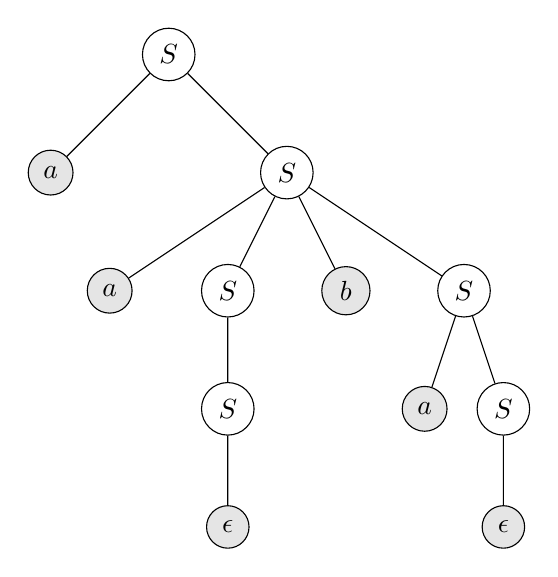
\begin{tikzpicture}[
				level/.style={sibling distance=30mm/#1},
				leaf/.style={circle, draw=black, fill=black!10},
				node/.style={circle, draw=black}
				]
			\node [node] {$S$}
				child {node [leaf] {$a$}}
				child {node [node] {$S$}
					child{node [leaf] {$a$}}
					child{node [node] {$S$}
						child{node [node] {$S$}
							child{node [leaf] {$\epsilon$}}}
					}
					child{node [leaf] {$b$}}
					child{node [node] {$S$}
						child{node [leaf] {$a$}}
						child{node [node] {$S$}
							child{node [leaf] {$\epsilon$}}
						}
					}
				};
			\end{tikzpicture}\\
		\end{center}

		Variante 2 (f�r das Wort $aaba$):
		\begin{center}
			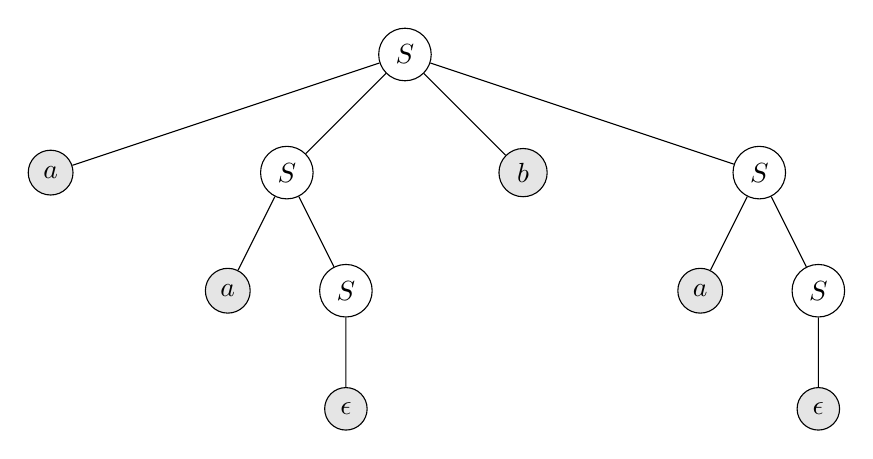
\begin{tikzpicture}[
				level/.style={sibling distance=30mm/#1},
				leaf/.style={circle, draw=black, fill=black!10},
				node/.style={circle, draw=black}
				]
			\node [node] {$S$}
				child {node [leaf] {$a$}}
				child {node [node] {$S$}
					child {node [leaf] {$a$}}
					child {node [node] {$S$}
						child {node [leaf] {$\epsilon$}}}}
				child {node [leaf] {$b$}}
				child {node [node] {$S$}
					child {node [leaf] {$a$}}
					child {node [node] {$S$}
						child {node [leaf] {$\epsilon$}}}};
			\end{tikzpicture}\\			
		\end{center}
		Da es mindestens zwei M�glichkeiten gibt, ist $G_{Auf}$ mehrdeutig.
		\end{solutionordottedlines}
		
		\part �ber linksseitige Ableitungen
		\begin{solutionordottedlines}[2cm]
		Variante 1 (f�r das Wort $aaba$):
		\begin{equation*}
			S \rightarrow aS \rightarrow aaSbS \rightarrow aa\epsilon bS \rightarrow aa\epsilon baS \rightarrow aa\epsilon ba\epsilon \rightarrow aaba
		\end{equation*}
		Variante 2 (f�r das Wort $aaba$):
		\begin{equation*}
			S \rightarrow aSbS \rightarrow aaSbS \rightarrow aa\epsilon bS \rightarrow aa\epsilon baS \rightarrow aa\epsilon ba\epsilon \rightarrow aaba
		\end{equation*}
		Wie im Parsebaum ist hier der erste Schritt ein anderer.
		\end{solutionordottedlines}

		\pagebreak
		\part �ber rechtsseitige Ableitungen
		\begin{solutionordottedlines}[2cm]
		Variante 1 (f�r das Wort $aaba$):
		\begin{equation*}
			S \rightarrow aS \rightarrow aaSbS \rightarrow aaSbaS \rightarrow aaSba\epsilon \rightarrow aa\epsilon ba\epsilon \rightarrow aaba
		\end{equation*}
		Variante 2 (f�r das Wort $aaba$):
		\begin{equation*}
			S \rightarrow aSbS \rightarrow aaSbS \rightarrow aaSbaS \rightarrow aaSba\epsilon \rightarrow aa\epsilon ba\epsilon \rightarrow aaba
		\end{equation*}
		Hier sind ebenfalls die ersten beiden Schritte vertauscht.
		\end{solutionordottedlines}

	\end{parts}

\end{questions}

